\section{Specifica}
\subsection{Introduzione}
La suite ASCON fornisce la cosiddetta \textbf{Authenticated Encryption with Associated Data (AEAD)}, nonché le funzionalità di hashing già citate.
\newline
Un cifrario autenticato consiste in uno schema di cifratura che possa assicurare, oltre alla più ovvia confidenzialità dei dati cifrari, l'integrità di questi, affinché il ricevente possa assicurarsi che il messaggio durante il transito non abbia subito distorsioni, dovute a disturbi o più importante a tampering da parte di un'entità terza. ASCON assicura l'integrità del messaggio trasmesso, nonché di eventuali dati associati. L'idea alla base è quella di restituire, al termine della cifratura, un \textbf{tag} da 128 bit estratto dallo state alla fine della procedura di cifratura. Lo state utilizzato per la cifratura, con riferimento ai diagrammi più avanti riportati, dipende anche da eventuali dati associati. In questo modo si può assicurare l'inegrità anche di quei metadati per i quali non è necessaria la confidenzialità, ma per i quali ci si vuole comunque assicurare dell'assenza di manipolazioni da parte di threat actors.
\newline\newline
Tutti gli schemi si basano su una funzione $p$, composta da somme, sostituzioni e permutazioni (più avanti approfondite) e che opera su una matrice di stato da 320 bit. La funzione è stata ideata per assicurare robustezza a fronte delle limitazioni hardware e software che un sistema embedded può imporre. Le operazioni sono \textbf{definite su parole da 64 bit} e trattandosi di \textbf{operazioni logiche} (AND, NOT, XOR, ROT), l'implementazione dello schema risulta particolarmente ottimale per ambienti di questo tipo. Inoltre, si adatta particolarmente a scenari in cui dispositivi trasmettono poche informazioni in maniera periodica: dai benchmark risulta che lo schema è particolarmente efficiente per messaggi brevi.
\newline\newline
Non vi è necessità di operazioni inverse, dal momento in cui $p^a$ e $p^b$ sono valutati in una sola diretazione sia per cifratura che decifratura. 
\newline\newline
ASCON non utilizza key scheduling o espansione di chiave. Non ci sono costi aggiuntivi quando la chiave viene cambiata. 
\subsubsection{Authenticated Encryption}
Per realizzare la cifratura con autenticazione dei dati gli algoritmi in ASCON sono parametrizzati tramite:
\begin{itemize}
    \item Lunghezza della chiave $k < 160$ bits
    \item Rate (dimensione del blocco) $r$
    \item Numero di round interni $a$ e $b$
\end{itemize}
Così facendo ogni schema definisce la propria funzione di cifratura $\epsilon_{k, r, a, b}$ e decifratura $D_{k, r, a, b}$. La procedura di cifratura prende in input una chiave $K$, un \textsl{nonce} $N$ da 128 bit, eventuali dati associati $A$ ed un plaintext $P$ di lunghezza arbitraria. Restituisce un ciphertext $C$ della medesima lunghezza del plaintext. Dunque
\[\epsilon_{k,r,a,b}(K,N,A,P)=(C,T)\]
La procedura di decifratura restituisce un plaintext se e solo se l'integrità è assicurata, ovvero previa uguaglianza del tag ricevuto e del tag ricacolato
\[D_{k,r,a,b}(K,N,A,C,T)\in\{P, \bot\}\]
\subsubsection{Hashing}
TODO

\subsubsection{Parametri}
Per quanto riguarda i parametri suggeriti:
\begin{table}[h!]
    \centering
    \begin{tabular}{|c|c|c|c|c|c|c|c|}
        \hline
        \textbf{Nome}       & \textbf{Algoritmo}            & \textbf{k} & \textbf{nonce} & \textbf{tag} & \textbf{blocco} & \textbf{a} & \textbf{b} \\
        \hline
        \textsl{ASCON-128}  & $\epsilon, D_{128, 64,12,6}$  & 128        & 128            & 128          & 64              & 12         & 6          \\
        \hline
        \textsl{ASCON-128a} & $\epsilon, D_{128, 128,12,6}$ & 128        & 128            & 128          & 128             & 12         & 8          \\
        \hline
    \end{tabular}
\end{table}

\subsubsection{State}
Tutti i design della suite utilizzato uno state da 320 bit, gestito tramite 5 parole da 64. Lo state viene aggiornato con la funzione $p$, ripetuta $a$ o $b$ volte in base alla fase in cui ci si trova (inizializzazione, cifratura/decifratura, finalizzazione). 

\subsection{Authenticated Encryption}
La modalità utilizzata da ASCON è basata sulle modalità \textbf{duplex} come \textsl{MonkeyDuplex} e \textsl{Sponge-based} design, seppur utilizzi una \textbf{inizializzazione} e \textbf{finalizzazione} (entrambe basate su chiave) più robuste. L'operazione di cifratura e decifratura avviene come in figura: 
\begin{figure}[h!]
    \centering
    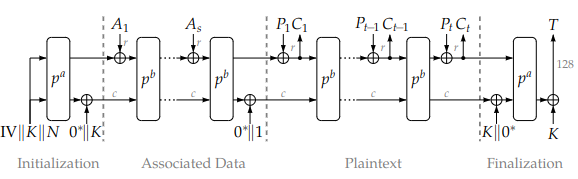
\includegraphics[width=12cm]{images/enc.png}
    \caption[short]{$\epsilon_{k,r,a,b}$}
\end{figure}
\begin{figure}[h!]
    \centering
    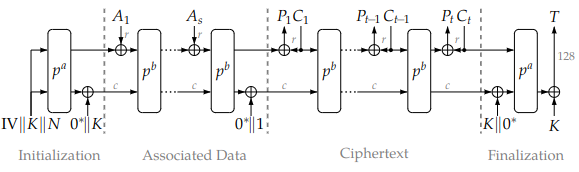
\includegraphics[width=12cm]{images/dec.png}
    \caption[short]{$D_{k,r,a,b}$}
\end{figure}
\paragraph*{Inizializzazione}
L'inizializzazione prevede uno state di partenza con la seguente forma: 
\[S \leftarrow IV_{k,r,a,b} || K || N\]
\[IV_{k,r,a,b} \leftarrow k || r || a || b || 0^{160-k} = 80400c0600000000\;\;\;\;per\;ASCON-128\]
L'inizializzazione si conclude con:
\[S\leftarrow p^a(S)\oplus (0^{320-k} || K)\]
\paragraph*{Dati associati}
I dati associati sono processati in blocci da $r$ bit. L'eventuale padding viene realizzando con l'append di un 1 finale ed il minor numero di 0 necessari per raggiungere una lunghezza che sia multiplo di $r$. Nel caso in cui non ci dovessero essere dati associati, si passa direttamente alla fase di cifratura/decifratura. Ogni blocco di dato associato viene messo in XOR con i bit più significativi dello state e la porzione di state sostituita con il risultato. Questo implica che il tag finale dipenderà anche dal valore dei dati associati e la verifica fallirà a fronte di un tampering di questi. 
\newline\newline
Alla fine di questa fase, lo state viene messo in XOR con 1 come costante di separazione del dominio. Questa operazione è svolta come contromisura di alcuni attacchi che potrebbero cambiare il ruolo dei blocchi di plaintext e dati associati. 
\paragraph*{Cifratura/Decifratura}
Come per i dati associati il plaintext/ciphertext viene suddiviso in blocchi con eventuale 1 + padding. Durante la cifratura, ad ogni XOR lo state viene aggiornato con il risultato dell'operazione. L'ultimo blocco di ciphertext viene troncato alla lunghezza dell'ultimo blocco di plaintext senza padding, in modo tale da preservare la lunghezza originale del messaggio. Si riapplica $p^b$ dopo ogni XOR ad eccezione dell'ultimo. 
\newline\newline
Per la decifratura invece il blocco di ciphertext viene inserito nello state ed utilizzato per effettuare uno XOR, in modo da recuperare il plaintext originale. Si riapplica $p^b$ dopo ogni XOR ad eccezione dell'ultimo. 
\newline\newline
Si noti come in assenza di dati associati e in presenza di un singolo blocco di plaintext da cifrare, non sono necessarie altre $p^b$ sullo state. Per prevenire lo scenario in cui lo XOR della chiave si cancelli, lo XOR viene effettuato su due parti dello state diverse. 
\paragraph*{Finalizzazione}
Durante la finalizzazione la chiave $K$ viene XORata con lo state, per poi applicare $p^a$. Si estrae dunque il tag $T$ dai 128 bit meno significativi dello state XORati con la chiave $K$. 
\subsection{Funzione p}
La funzione $p$ introduce le proprietà di confusione, tramite S-Box, e diffusione, tramite il linear layer. Ogni round $p$ è un SPN-based round.  
\begin{figure}[h!]
    \centering
    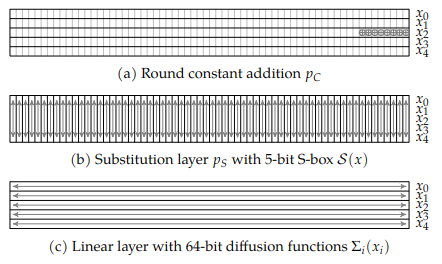
\includegraphics[width=10cm]{images/p.png}
\end{figure}
\begin{figure}[h!]
    \centering
    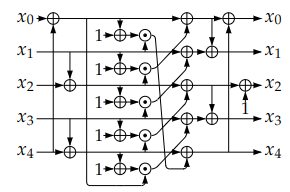
\includegraphics[width=6cm]{images/sbox.png}
    \caption[short]{Approccio bitsliced per applicazione della S-Box}
\end{figure}
\newline
La prima operazione svolta è uno XOR con una costante. La costante è identificata dal numero di round in cui ci si trova. Si passa poi alla sostituzione tramite S-Box, la cui implementazione è preferibile nella sua forma \textsl{bitsliced} con operazioni effettuate sulle intere parole da 64 bit. Infine si passa al layer di diffusion, dove ad ogni parola da 64 bit si applicano degli XOR con la medesima parola ruotata di un determinato numero di bit a destra. 
\paragraph*{Costante di round}
Le costanti di round sono state scelte grandi abbastanza per evitare \textsl{slide, rotational, sel-fimilarity} o attacchi simili. La scelta è stata effettuata in maniera semplice, ovvero incrementando o meno un counter. La posizione invece è stata scelta per permettere il pipelining con le operazioni precedenti e successive (ad esempio le istruzioni successive per le S-box). 
\paragraph*{Sobstitution layer}
Il layer di sostituzione è l'unica porzione non lineare del round. Mixa i 5 bit che compongono una colonna nello state.

\subsection{ASCON-128}
Si tratta di un cifrario a blocchi che prevede operazioni di sostituzione e permutazione, nonché di somma e rotazioni di bit. Come accennato tutte le operazioni sono ripetute in più round ed implementate unicamente tramite bitwise operations.

\newpage